\chapter{Classification techniques}
\label{ch:ClassificationTechniques}

\section{Introduction}
This chapter deals with the statistical foundations of species distribution modelling. Since it is impractical to list all the available methods that are used we restrict ourselves to the most popular or fundamental ones. In the last 10 years a lot of research has focused on the performance of these different algorithms \parencite[e.g.][]{elith*_novel_2006,segurado_evaluation_2004}. The results of these studies were taken into account when the methods that are used were selected.

\section{Presence-absence data}
\label{sec:PresenceAbsenceDta}

In this section some important and often used methods to classify binary data are reviewed. First of all, the outcome, $y_i$, of observation $i$ indicates whether a species occurs, $y_i = 1$, or is absent, $y_i=0$. We denote the vector of explanatory variables as $\bm{X}$. The general form of the models used in this section is:
\begin{equation}
\label{FundEq}
P(Y=1|\bm{X} = \bm{x}) = f(\bm{x}; \bm{\gamma}).
\end{equation}
In this representation $f(\cdot;\cdot)$ is a function parametrized by $\bm{\gamma}$. The main differences between the techniques introduced below are the functional form of $f(\cdot;\cdot)$ and the loss function that is minimized.

\subsection{Logistic regression}
Perhaps the most fundamental modelling technique for binary data is logistic regression. In logistic regression the log odds ratio of the probability of an occurrence is modelled as a linear function of the covariates. Hence, the model can be depicted as \[\log \left( \frac{P(Y=1|\bm{X} = \bm{x})}{P(Y=0|\bm{X} = \bm{x})} \right)= \bm{x}^t \bm{\gamma}.\]
It is easy to show that this model can be written in the form used in Equation \ref{FundEq}. More specifically, if we define $\expit(\cdot) = \frac{\exp(\cdot)}{1+\exp(\cdot)}$ we get \[f(\bm{x};\bm{\gamma}) = \expit(\mathbf{x}^t\bm{\gamma}).\] Usually the coefficients of a logistic regression model are obtained by using maximum likelihood estimation (MLE). Obtaining the MLE $\widehat{\bm{\gamma}}$ corresponds with solving the following maximization problem:
\[\widehat{\bm{\gamma}} = \argmax_{\bm{\gamma}} \sum_{i=1}^{N} \left\lbrace y_i \log{f(\bm{x}_i;\bm{\gamma})}  + (1-y_i)\log{f(\bm{x}_i;\bm{\gamma})}  \right\rbrace.\] 
When one multiplies this log-likelihood function by minus one we get a loss function that is often called the cross-entropy. For more information about logistic regression and numerical optimization techniques for obtaining the MLE we refer to \cite{agresti_categorical_2013} and \cite{mccullagh_generalized_1999}. \\

The main advantages of logistic regression models are that they are relatively simple to implement, interpret, etc. This simplicity is also its greatest disadvantage. In particular, when modelling the distribution of a species there is often no a priori knowledge of the shape of the response curves.

\subsection{Generalized additive models}
\label{sec:GAM}
In standard logistic regression a linear systematic component is used. It is easy to extend logistic regression models to include non-linear systematic components. However, the functional form of the log odds ratio might not be known by the researcher and hence a non-parametric (or semi-parametric) modelling technique can be useful. When the distribution of the outcome belongs to the exponential family generalized additive models (GAMs) are one possible class of non-parametric (or semi-parametric) models. In the case of a Bernoulli distribution the resulting GAM is sometimes called an additive logistic regression model and has the form:
\begin{equation}
\label{GAMs}
\log \left( \frac{P(Y = 1|\bm{X} = \bm{x} )}{P(Y=0|\bm{X} = \bm{x})} \right) = \gamma_0 + f_1(x_{1}) + \dots + f_p(x_{p}).
\end{equation}
In this representation the $f_k(\cdot)$'s are certain smooth functions. Again one can write this model in the form of Equation \ref{FundEq}:
\[f(\bm{x};\bm{\gamma}) = \gamma_0 + f_1(x_{1}) + \dots + f_p(x_{p})\] 
There is a multitude of popular ways to specify the $f_k(\cdot)$'s \parencite{wood_generalized_2006, hastie_generalized_1990}. We will follow \cite{wood_generalized_2006} and \cite{wood_gams_2002} and focus on using cubic smoothing splines to represent the $f_k(\cdot)$'s. \\

GAMs are most often fitted by using MLE. In order to restrict the ``wiggliness'' of the smoothing functions in model \ref{GAMs} one can add a penalization term to the likelihood function. An example of such a ``wiggliness'' penalty is:
\[\sum_{j=1}^p \lambda_j \int_{x_{j(1)}}^{x_{j(n)}} \{f^{(2)}_j(x) \}^2dx.\]
In this penalization term the $x_{j(1)}$ (resp.\ $x_{j(n)}$) is the smallest (resp.\ largest) value of the $j$'th covariate. Furthermore, it can be shown that, in a class of sufficiently smooth functions, the minimizer of
\[- \sum_{i=1}^{N} \left\lbrace y_i \log{f(\bm{x}_i;\bm{\gamma})}  + (1-y_i)\log{f(\bm{x}_i;\bm{\gamma})} \right\rbrace + \sum_{j=1}^p \lambda_j \int_{x_{j(1)}}^{x_{j(n)}} \{f_j^{(2)}(x)\}^2 dx\]
is a natural cubic spline with knots at the $n$ covariate values. The two limiting cases, $\lambda = 0$ and $\lambda = \infty$, are interesting. If $\lambda = 0$ an interpolating spline is optimal, while when $\lambda \to \infty$ the solution converges to the linear logistic regression solution. Finally, fitting GAMS with natural cubic splines as smoothing functions is, compared to most other smoothers used in GAMS, computationally efficient.\\

In practice we have to select the penalization parameters, this is usually done by using cross-validation. Because the fitting procedures for GAMs are often computationally intensive usually the closely related generalized cross-validation (GCV) is used \parencite{wood_gams_2002}. Finally, since $\lambda = \infty$ still allows a first order fit, it can be interesting to perform additional model selection. Although variable selection is the topic of Chapter \ref{ch:ReducingTheNumberOfExplanatoryVariables} we mention that it is possible to introduce an extra penalization term that leads to an automatic variable selection technique \parencite{marra_practical_2011}, i.e.\ might remove a predictor from the model. This approach is implemented in the \textsc{mgcv} R package \parencite{mgcv}. \\

Finally, up till now only univariate splines have been considered, if interaction terms are to be included one can use e.g.\ thin plate splines. However, using multidimensional splines usually results in a computationally intensive fitting procedure. Finally, for a more applied review of the use of GAMs in species distribution modelling we refer to \cite{guisan_generalized_2002}.

\subsection{Artificial neural networks}
Artificial neural networks (ANNs) are a non-linear modelling technique. We refer to \cite{bishop_neural_1995} for an introduction to the general methodology and some of the technical details. The terminology used in the ANN literature is slightly different than in the standard statistical literature. More particularly, the explanatory variables are usually called the input features. Furthermore, an ANN consists of so-called ``layers'' of ``neurons'. The first layer is called the input layer and consists of one neuron for each variable. In each successive layer the output of the corresponding neurons is the result of applying an activation function, $g(\cdot)$, to a linear combination of the values from the previous layer. The coefficients of these linear combinations are called the weights of the ANN. These weights are the parameters one can tune. The process of feeding the values of the previous layer into the next is repeated up to the last layer which is called the output layer. The layers that are neither the input nor output layer are called hidden layers. A graphical representation of an ANN with one hidden layer can be found in Figure \ref{fig:chClassificationTechniques:ANN}.\\

\begin{figure}[!htb]
\centering
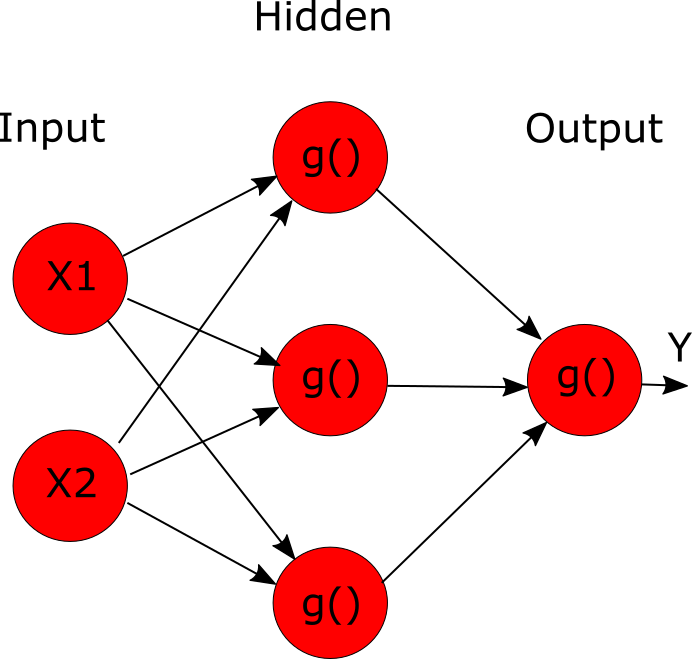
\includegraphics[scale=0.3]{VectorGraphics/ANN.png}
\caption{\label{fig:chClassificationTechniques:ANN}Visualization of a feed-forward neural network with one hidden layer.}
\end{figure}

From here on we will denote the vector of all the weights as $\bm{\gamma}$. As usual, the estimated weights are obtained by minimizing a loss function. When ANNs are applied to classification problems often either the squared loss, $L(\bm{y};\bm{\gamma}) = \sum_i (y_i - f(\bm{x}_i;\bm{\gamma}))^2$ or the cross-entropy, $L(\bm{y};\bm{\gamma}) = - \sum_i \left[ y_i \log \{ f(\bm{x}_i;\bm{\gamma})\} + (1-y_i)\log \{f(\bm{x}_i;\bm{\gamma})\}\right]$ is used. We will use the cross-entropy since it is closely related to the likelihood of a Bernoulli distribution and hence more in line with the other techniques. To minimize the loss criterion, often backpropagation \parencite{rumelhart_learning_1986} is used in combination with a numerical optimization algorithm, e.g.\ steepest descent. \\

It is easy to see that logistic regression can be seen as an ANN with: no hidden layers, the expit function as the activation function of the output layer, and the cross-entropy loss.\\

The biggest strength of ANNs is that, under some regularity constraints, they can approximate any continuous function arbitrarily well \parencite{hornik_multilayer_1989}. Some disadvantages include:
\begin{itemize}
\item Selecting an optimal number of layers and neurons is far from trivial.
\item The loss-function often has multiple local minima.
\item Different numerical optimization methods often lead to different solutions.
\item Fitting large neural network architectures can be computationally infeasible.
\item The backpropagation algorithm cannot be used in combination with non-differentiable penalty functions, e.g.\ the lasso penalty (see Section \ref{sec:Lasso}).
\item The fitted parameters can be sensitive to the initial weights.
\item The obtained model seems like a ``black-box'', i.e. there is often no easy way to interpret the parameters and the effect of different predictors.
\end{itemize}
Some of these disadvantages can be, partially, overcome by using e.g.\ weight decay, averaging networks, early stopping, pruning, \dots\ Weight decay is also referred to as $L_2$ regularization and is described in Section \ref{sec:L2Regularization}. Averaging networks boils down to using different sets of initial values, fitting the same network structure for each set, and then combining these into one model \parencite{ripley_pattern_2009}. The \textsc{caret} package \parencite{caret} provides an implementation of averaged neural networks based upon the \textsc{nnet} package \parencite{nnet}.


\subsection{Tree based methods}
In this section some tree based methods are introduced.  The section starts with a short explanation of decision trees. Afterwards boosting is introduced as a method to deal with some of the shortcomings of decision trees.

\subsubsection{Decision trees}
\label{sec:DecisionTrees}
Tree based methods are a class of algorithms that partition the input space into rectangular regions. The same predicted value is then assigned to all observations within a certain region. In the context of SDMs we can interpret this as partitioning the environmental space into rectangles. Each of these rectangles is then labelled as being part of the niche or not. To obtain such rectangles we start by splitting the input space into two regions along one variable. The variable and the value that is used to obtain this split is selected in such a way that the loss function of interest is minimized. In the following steps either the algorithm stops if some stopping criterion is met or the obtained sub-regions are split into smaller sub-regions. After the tree is grown usually a winner takes all approach is applied to obtain the label for each region. Thus, if a region contains mainly presences its predicted class will be the presence class, otherwise it will be labelled as a region containing absences. Finally, the number of nodes $J$ of a tree is defined as the number of splits $+1$. A visualization of a partitioning obtained bys using a classification tree is given in Figure \ref{fig:chClassificationTechniques:CART}. \\

\begin{figure}[!htb]
\centering
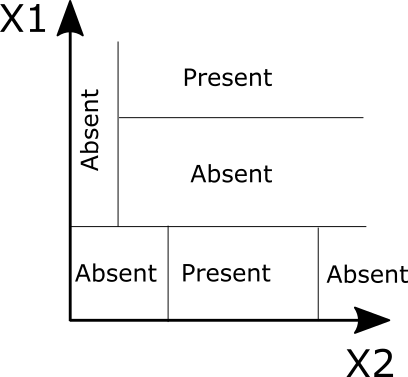
\includegraphics[scale=0.5]{VectorGraphics/CART.png}
\caption{\label{fig:chClassificationTechniques:CART}Visualization of a classification tree in a two dimensional input space.}
\end{figure}

Unless a stopping criteria is specified this approach would lead to over-fitting. More particularly we would end up with as many regions as there are observations. Hence, the algorithm is usually stopped when no new splits can be found that decrease the loss by some pre-specified amount. Another possible stopping criterion is to stop the algorithm once a certain number of splits is reached. As usually we opt for using the cross-entropy as the loss function. Finally, we note that there are many variations to the algorithm sketched above.

The most important advantages of decision trees include:
\begin{itemize}
\item Complex interaction effects can easily be modelled.
\item Small decision trees are easily visualized.
\item Decision trees usually perform relatively well even when no variable selection was applied.
\item The idea underlying decision trees is quite intuitive.
\item Decision trees are invariant under monotonic transformations of the predictors.
\end{itemize}

Some of the disadvantages of using decision trees include:
\begin{itemize}
\item Decision trees usually have a large variance
\item Categorical variables with a lot of classes can lead to computational problems.
\end{itemize}

\subsubsection{Boosting}
\label{sec:Boosting}
In order to combat the large variance of decision tree boosting was introduced. The overview of boosting presented in this section is largely based on \cite{elith_working_2008} and \cite{friedman_additive_2000}. \cite{elith_working_2008} gave an applied working guide to boosted regression trees while \cite{friedman_additive_2000} gave a theoretical explanation of boosted regression trees.\\

An ensemble of different classifiers is sometimes useful to obtain improved classifiers. This is what is done in boosted classification trees. Boosting can be described as creating a sequence of models such that the $i$'th model focusses on correctly classifying observations that were misclassified by the $i-1$ previous models. The corresponding algorithm then takes the following form:\\
\begin{enumerate}
\item Construct a classifier.
\item Classify the observations.
\item Assign large weights to wrongly classified observation and vice versa for correctly classified observations. 
\item Fit a classifier on the weighted data-set.
\item Create a new classifier by adding the the new and old classifiers, usually the new classifier is shrunken by multiplying it with a regularization parameter.
\item Stop if some stopping criteria is met, otherwise use the new classifier obtained in step 5. and repeat from step 2. onwards.
\end{enumerate}

In order to avoid over-fitting one can use a new subsample of the full data-set in each iteration of the algorithm. When combining boosting with classification trees it is recommended that the subsamples have a sample size in between $0.5$ and $0.75$ times the size of the full dataset \parencite{elith_working_2008}.\\

Another popular ensemble method that is used in combination with decision trees is the Random Forest (RF) method. In most cases RFs perform slightly worse than boosted classification trees \parencite{hastie_elements_2009} and we will not consider them in this thesis.\\

A disadvantage of Boosted classification trees is that they are not as easily visualized / interpreted as normal classification trees. Secondly, there are quite a few tuning parameters, namely the depth of the trees $J$, the regularization term, and the number of trees. However, \cite{hastie_elements_2009} note that using $J \in \{4,\dots,8\}$ usually leads to the best performing models, additionally they observed that the specific value of $J$ in this set has little effect on the performance of the classifier. Hence, cross validation will be used to obtain optimal values for the learning rate and the number of trees.\\

Finally, although we described boosting for classification trees the same idea can be readily applied to other classification algorithms. Furthermore, boosted classification trees seem to include a form of internal variable selection, i.e.\ the performance of this method usually doesn't degrade a lot when irrelevant predictors are present. We will use the implementation provided by the \textsc{gbm} package \parencite{gbm}.

\section{Presence-only data}
\label{sec:PresenceOnlyData}
Instead of having access to presence-absence data it happens quite often that we only have presence data. This is e.g. the case when we use the records of a natural history museum, herbarium, \dots One method of dealing with this kind of data is by extending the methods from Section \ref{sec:PresenceAbsenceData}, this is done in Section \ref{sec:ClassificationWithPseudoAbsences}. Another popular approach is Maximum Entropy modelling \parencite{phillips_maximum_2006,phillips_modeling_2008}, a short overview of this method is given in Section \ref{sec:MaximumEntropyModeling}. Finally we refer to \parencite{pearce_modelling_2006} for different methods to deal with and additional information on presence-only data. 

Finally, there is another interesting way to use regression models in combination with presence-only data. \cite{ward_presence-only_2009} used the EM algorithm \parencite{dempster_maximum_1977} in combination with regression models. Although this leads to an elegant and rigorously motivated method of fitting regression models the prevalence of the species needs to be known, or estimable, which is (nearly) never the case.

\todo[inline]{unify MaxEnt / pesudo-absences by introducing IPP models}
\subsection{Classification with pseudo-absences}
\label{sec:ClassificationWithPseudoAbsences}
\todo[inline]{connection with IPP models}
\todo[inline]{discuss the possibility of using weighted data (e.g. for decision trees etc.) see paper.}
\todo[inline]{Read/find some papers on classification methods with unbalanced data-sets.}
\todo[inline]{discuss effect of using PCA on background vs occurrence data}





\subsection{Maximum Entropy modelling}
\label{sec:MaximumEntropyModeling}
Perhaps the most popular method to create models from presence-only data is by using Maximum Entropy modelling \parencite[MaxEnt][]{phillips_maximum_2006,phillips_modeling_2008}. This introduction follows the interpretation introduced by \cite{elith_statistical_2011} instead of the original motivation of \cite{phillips_maximum_2006}. This is done mainly because in our opinion it is the most intuitive explanation of the algorithm. \\

Usually the MaxEnt algorithm is applied to raster data (however this is not necessary). The extent of the raster defines the study are $L$. Since we usually know the covariate values $\bm{z}$ of each cell (using e.g.\ GIS layers) we can define a probability distribution of the covariates $f(\bm{z})$ which is implied by defining a uniform distribution over $L$. We then try to find the distribution $f_1(\bm{z})$ of the features of the cells where a presence was recorded. This distribution is defined as the distribution which minimizes the Kullback-Leibler divergence with respect to $f(\bm{z})$ and such that the mean of values of the features (with respect to $f_1{z}$) are close to the empirical means of the presence sites.\\

The standard implementation of MaxEnt uses as features a combination of products between covariates, hinge features, step functions, quadratic terms and linear terms \parencite{phillips_modeling_2008}. To avoid over-fitting a regularization term is added, more particularly a lasso penalty (see Section \ref{sec:Lasso}). \\

Advantages include:
\begin{itemize}

\item MaxEnt has been shown to perform well in a variety of comparative studies \parencite[e.g.][]{elith*_novel_2006}.
\end{itemize}

Some main disadvantages are:
\begin{itemize}
\item The output and interpretation is dependent on the scale of the cells.
\item MaxEnt is perceived as a black-box model.
\item No standard errors are available.
\item There are few model checking tools available.
\end{itemize}
However, most of these problems can be ``solved'' by utilizing the connection with inhomogeneous poison models \parencite[IPP,][]{renner_equivalence_2013,fithian_finite-sample_2013}, yet this equivalence is rarely used in practice and as of yet not implemented in the standard MaxEnt software.

\section{Taking the scale hierarchy into account}
\label{sec:TakingTheScaleHierarchyIntoAccount}
In Section \ref{sec:SpatialScale} the influence of spatial scale was discussed. There have been some attempts to incorporate this hierarchical structure into the classification techniques. E.g.\ \cite{pearson_modelling_2004} combined two models, one for coarse scale processes and one that introduces fine grain variables. More specifically their approach was as follows: \\
\begin{enumerate}
\item An initial model is obtained by solely using climate variables as predictors.
\item The predicted values are saved as a new variable.
\item The predicted values and remote sensed variables are combined and used as the input for a second model.
\item The predicted values of the second model are the final predictions.
\end{enumerate}

Graphically this can be depicted as in Figure \ref{fig:chClassificationTechniques:HierarchicalClassification}.\\

\begin{figure}[!htb]
\centering
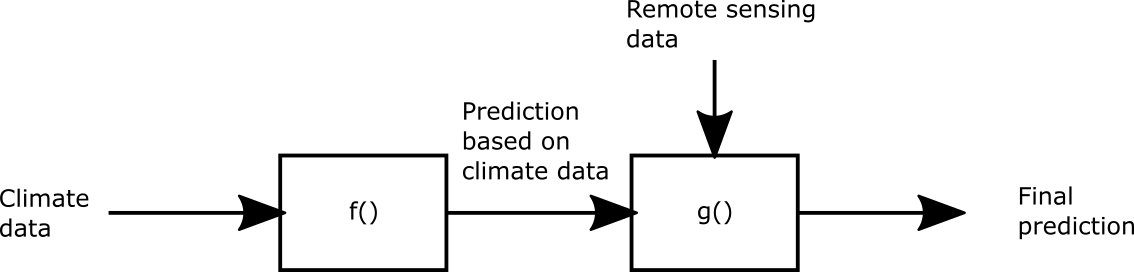
\includegraphics[scale=0.5]{VectorGraphics/HierarchicalClassification.png}
\caption{\label{fig:chClassificationTechniques:HierarchicalClassification}Visualization of the hierarchical model.}
\end{figure}

This hierarchical model has since been applied in combination with e.g.\ stacked SDMs \parencite{cord_remote_2014}. However, from a statistical point of view this approach is not well motivated. The main drawback of this approach is that interaction effects between the climate and remotely sensed variables cannot be taken into account. Furthermore, since there is usually quite some correlation between the climate and remotely sensed variables model selection is hampered. For example, if a remotely sensed variable is fundamental in determining the niche and highly correlated with a climate variable that is not as relevant for defining the niche the climate variable will usually end up in the model instead of the remotely sensed variable. Because of these drawbacks this approach will not be investigated.







